\documentclass[resume]{subfiles}


\begin{document}
\section{Basses fréquences}
\begin{itemize}
\item $\vec{E}$ : Champ électrique [\si{\volt\per\meter}]
\item $\vec{D}$ : Déplacement (ou induction) électrique [\si{\coulomb\per\square\meter}] ou [\si{\ampere\second\per\square\meter}]
\item $\vec{H}$ : Champ magnétique [\si{\ampere\per\meter}]
\item $\vec{B}$ : Induction magnétique [\si{\tesla}] ou [\si{\volt\second\per\square\meter}]
\item $\vec{J}$ : Densité de courant [\si{\ampere\per\square\meter}]
\item $\vec{A}$ : Potentiel vecteur [\si{\tesla\meter}] ou [\si{\weber\per\meter}]
\item $\Phi$ : Flux d'induction magnétique [\si{\weber}]
\item $\varepsilon$ : permittivité [\si{\farad\per\meter}]
\item $\mu$ : perméabilité [\si{\henry\per\meter}]
\item $\sigma$ : conductivité [\si{\siemens\per\meter}]
\end{itemize}
\paragraph{Isovaleur} : Ligne sur laquelle la valeur est constante
\paragraph{Ligne de champ} : Ligne sur laquelle les vecteurs sont tangents
\begin{itemize}
\item $D$ est la conséquence de $E$ (tension)
\item $B$ est la conséquence de $H$ (courant)
\end{itemize}
\begin{itemize}
\item Sources en électrostatique : charges ou potentiels
\item Sources en magnéto statique : courant ou aimant
\end{itemize}



\subsection{Équations de Maxwell}
$$\Rot\vec{E}=-\frac{\partial \vec{B}}{\partial t}$$
$$\Rot\vec{H}=\vec{J}+\frac{\partial \vec{D}}{\partial t}$$
$$\Div\vec{D}=\rho$$
$$\Div\vec{B}=0$$
\subsection{Relations spécifiques aux matériaux}
$$\vec{B}=\mu_0\mu_r\vec{H}$$
$$\vec{D}=\varepsilon_0\varepsilon_r\vec{E}$$
$$\vec{J}=\sigma\vec{E}$$
\subsection{Flux}
Intégrale sur une surface
$$\iint_s\vec{F}d\vec{S}$$
\subsection{Potentiel}
$$U_{AB}=\int_{A}^{B}\vec{E}d\vec{l}$$
\subsection{Gradient}
$$\vec{\text{grad}}f=\grad f=\frac{\partial f}{\partial x}\vec{i}+\frac{\partial f}{\partial y}\vec{j}+\frac{\partial f}{\partial z}\vec{k}$$
C'est la direction dans laquelle la fonction varie le plus. Le gradient est toujours perpendiculaire aux lignes d'isovaleurs.
\subsection{Divergence}
$$\Div\vec{F}=\nabla \vec{F}=\frac{\partial F_x}{\partial x}+\frac{\partial F_y}{\partial y}+\frac{\partial F_z}{\partial z}$$
La divergence traduit une "création" ou une "destruction" de vecteurs.
\subsection{Rotationnel}
$$\Rot \vec{F}=\nabla \times \vec{F}=\left(\frac{\partial F_z}{\partial y}-\frac{\partial F_y}{\partial z}\right)\vec{i}+\left(\frac{\partial F_x}{\partial z}- \frac{\partial F_z}{\partial x}\right)\vec{j}+\left(\frac{\partial F_y}{\partial x}-\frac{\partial F_x}{\partial y}\right)\vec{k}$$
\subsubsection{Propriétés}
$$\Div(\Rot \vec{F})=0$$
\subsection{Laplacien}
$$\Div(\grad f)=\nabla^2 f=\frac{\partial^2 f}{\partial x^2}+\frac{\partial^2 f}{\partial y^2}+\frac{\partial^2 f}{\partial z^2}$$
\subsection{Propriétés}
$$\Div(\grad f)=\Delta f$$

\section{Modèles}
\subsection{Électrostatique}
$$\Rot\vec{E}=\vec{0}$$
$$\Div\vec{D}=\rho$$
$$\vec{D}=\varepsilon\vec{E}$$
La relation $\Rot\vec{E}=\vec{0}$ implique qu'il existe un potentiel scalaire tel que
$$\vec{E}=-\grad V$$
Équation de Poisson
$$\Delta V=\frac{-\rho}{\varepsilon}$$
Équation de Laplace (lorsqu'il y a pas de densité de charge, et par conséquent $\rho=0$) :
$$\Delta V=\frac{\partial^2V}{\partial x^2}+\frac{\partial^2 V}{\partial y^2}=0$$
\begin{itemize}
\item Dimensionnement d'un isolant
\item Mesure sans contact (capteur capacitif)
\end{itemize}

\subsection{Électrocinétique}
On s'intéresse à la façon dont le courant se déplace
$$\Rot\vec{E}=0$$
$$\Div\vec{D}=\rho$$
$$\Rot\vec{H}=\vec{J}$$
Comme pour l'électrostatique, on a
$$\vec{E}=-\grad V$$
On a aussi
$$\Div\vec{J}=0$$
L'équation à résoudre est
$$\sigma \Delta V=0$$
Utilisé pour des connecteurs
\subsection{Magnétostatique}
Courant fixe
$$\Rot\vec{E}=\vec{0}$$
$$\Rot\vec{H}=\vec{J}$$
$$\Div\vec{B}=0\qquad \vec{B}=\Rot\vec{A}$$
$$\vec{H}=\nu\vec{B}-\vec{H}_c$$
$$\nu=\frac{1}{\mu}$$
Équation de poisson :
$$\left(\frac{\partial A_z}{\partial x^2}+\frac{\partial A_z}{\partial y^2}+\frac{\partial A_z}{\partial z^2}\right)\vec{k}=-\mu J_z\vec{k}$$
Les sources sont :
\begin{itemize}
\item Des courants
\item Des aimants
\end{itemize}
Si on combine les relations on peut obtenir la relation de Poisson
$$\Delta \vec{A}=-\mu \vec{J}$$
Avec $\Delta$ le Laplacien
\begin{itemize}
\item Haut-parleurs
\item Capteur magnétique
\end{itemize}
\subsection{Magnéto-transitoire}
\begin{itemize}
\item Moteur et générateur électrique
\end{itemize}

$$\Rot{\vec{E}}=-\frac{\partial \vec{B}}{\partial t}$$
$$\Rot{\vec{H}}=\vec{J}$$
$$\Div{\vec{B}}=0$$
$$\vec{J}=\sigma\vec{E}\qquad \vec{H}=\nu\vec{B}-\vec{H}_c$$
$$\vec{B}=\Rot{\vec{A}}$$
$$\vec{E}=-\grad V-\frac{\partial \vec{A}}{\partial t}$$
Autres relations :
$$\Rot{\vec{E}}=-\Rot\left(\grad V\right)-\Rot\left(\frac{\partial \vec{A}}{\partial t}\right)=-\frac{\partial}{\partial t}\left(\Rot \vec{A}\right)=-\frac{\partial \vec{B}}{\partial t}$$
$$\Rot\left(\nu \Rot\vec{A}-\vec{H}_c\right)+\sigma\left(\grad V+\frac{\partial \vec{A}}{\partial t}\right)=0$$


\subsection{Magnéto-harmonique (courant sinusoïdal)}
\begin{itemize}
\item Capteur par courant de Foucault
\item Mesure non destructive
\item Effet de peau
\end{itemize}
\subsection{Symétries}
\begin{itemize}
\item A l'infini : $A=0$
\item Symétrie géometrique et antisymétrie physique : $A=0$
\item Symétrie géométrique et symétrie physique : $\frac{\partial A}{\partial n}=0$
\end{itemize}


$$\Rot \vec{E}=-\frac{\partial \vec{B}}{\partial t}$$
$$\Rot \vec{H}=\vec{J}$$
$$\Div \vec{B}=0$$
$$\vec{J}=\sigma \vec{E}\qquad \vec{H}=\nu \vec{B}$$
$$\vec{B}=\Rot \vec{A}$$
$$\vec{E}=-\grad V-\frac{\partial \vec{A}}{\partial t}$$
Autres relations :

$$\Rot\left(\nu \Rot\vec{A}\right)+\sigma\left(\grad V+\frac{\partial \vec{A}}{\partial t}\right)=0$$
$$\Rot\left(\nu \Rot\vec{A}\right)+\sigma\left(\grad V+j\omega \vec{A}\right)=0$$
\subsection{Loi de Snell}
\begin{figure}[H]
\centering
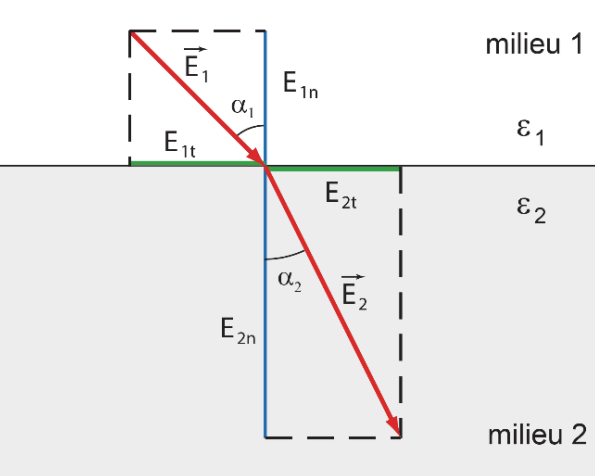
\includegraphics[width=4.00cm]{img_0.png}
\end{figure}
$$D_{1n}=D_{2n}$$
$$E_{1n}=\frac{\varepsilon_2}{\varepsilon_1}E_{2n}$$
$$\frac{E_{1n}}{E_{1t}}=\frac{\varepsilon_2}{\varepsilon_1}\frac{E_{2n}}{E_{2t}}$$
$$\tan\alpha_2=\frac{\varepsilon_2}{\varepsilon_1}\tan\alpha_1$$

\end{document}